\documentclass[10pt]{paper}\usepackage[]{graphicx}\usepackage[]{color}
%% maxwidth is the original width if it is less than linewidth
%% otherwise use linewidth (to make sure the graphics do not exceed the margin)
\makeatletter
\def\maxwidth{ %
  \ifdim\Gin@nat@width>\linewidth
    \linewidth
  \else
    \Gin@nat@width
  \fi
}
\makeatother

\definecolor{fgcolor}{rgb}{0.345, 0.345, 0.345}
\newcommand{\hlnum}[1]{\textcolor[rgb]{0.686,0.059,0.569}{#1}}%
\newcommand{\hlstr}[1]{\textcolor[rgb]{0.192,0.494,0.8}{#1}}%
\newcommand{\hlcom}[1]{\textcolor[rgb]{0.678,0.584,0.686}{\textit{#1}}}%
\newcommand{\hlopt}[1]{\textcolor[rgb]{0,0,0}{#1}}%
\newcommand{\hlstd}[1]{\textcolor[rgb]{0.345,0.345,0.345}{#1}}%
\newcommand{\hlkwa}[1]{\textcolor[rgb]{0.161,0.373,0.58}{\textbf{#1}}}%
\newcommand{\hlkwb}[1]{\textcolor[rgb]{0.69,0.353,0.396}{#1}}%
\newcommand{\hlkwc}[1]{\textcolor[rgb]{0.333,0.667,0.333}{#1}}%
\newcommand{\hlkwd}[1]{\textcolor[rgb]{0.737,0.353,0.396}{\textbf{#1}}}%
\let\hlipl\hlkwb

\usepackage{framed}
\makeatletter
\newenvironment{kframe}{%
 \def\at@end@of@kframe{}%
 \ifinner\ifhmode%
  \def\at@end@of@kframe{\end{minipage}}%
  \begin{minipage}{\columnwidth}%
 \fi\fi%
 \def\FrameCommand##1{\hskip\@totalleftmargin \hskip-\fboxsep
 \colorbox{shadecolor}{##1}\hskip-\fboxsep
     % There is no \\@totalrightmargin, so:
     \hskip-\linewidth \hskip-\@totalleftmargin \hskip\columnwidth}%
 \MakeFramed {\advance\hsize-\width
   \@totalleftmargin\z@ \linewidth\hsize
   \@setminipage}}%
 {\par\unskip\endMakeFramed%
 \at@end@of@kframe}
\makeatother

\definecolor{shadecolor}{rgb}{.97, .97, .97}
\definecolor{messagecolor}{rgb}{0, 0, 0}
\definecolor{warningcolor}{rgb}{1, 0, 1}
\definecolor{errorcolor}{rgb}{1, 0, 0}
\newenvironment{knitrout}{}{} % an empty environment to be redefined in TeX

\usepackage{alltt}


\usepackage{amsmath}
\usepackage{float}
\usepackage{amssymb}
\usepackage{geometry}

\title{Econometrics HW4}
\author{Timothy Schwieg}
\IfFileExists{upquote.sty}{\usepackage{upquote}}{}
\begin{document}
\maketitle

\begin{knitrout}
\definecolor{shadecolor}{rgb}{0.969, 0.969, 0.969}\color{fgcolor}\begin{kframe}
\begin{alltt}
\hlkwd{library}\hlstd{(sandwich)}
\hlstd{EngelData} \hlkwb{<-} \hlkwd{read.table}\hlstd{(} \hlstr{"Engel.dat"} \hlstd{)}

\hlkwd{summary}\hlstd{( EngelData )}
\end{alltt}
\begin{verbatim}
##        V1               V2        
##  Min.   : 377.1   Min.   : 242.3  
##  1st Qu.: 638.9   1st Qu.: 429.7  
##  Median : 884.0   Median : 582.5  
##  Mean   : 982.5   Mean   : 624.2  
##  3rd Qu.:1164.0   3rd Qu.: 743.9  
##  Max.   :4957.8   Max.   :2032.7
\end{verbatim}
\begin{alltt}
\hlstd{firstReg} \hlkwb{<-} \hlkwd{lm}\hlstd{( EngelData}\hlopt{$}\hlstd{V1} \hlopt{~} \hlstd{EngelData}\hlopt{$}\hlstd{V2 )}
\hlkwd{summary}\hlstd{( firstReg )}
\end{alltt}
\begin{verbatim}
## 
## Call:
## lm(formula = EngelData$V1 ~ EngelData$V2)
## 
## Residuals:
##     Min      1Q  Median      3Q     Max 
## -570.58 -106.12  -21.57   72.12 1916.37 
## 
## Coefficients:
##               Estimate Std. Error t value Pr(>|t|)    
## (Intercept)  -85.73632   34.58206  -2.479   0.0139 *  
## EngelData$V2   1.71146    0.05068  33.772   <2e-16 ***
## ---
## Signif. codes:  0 '***' 0.001 '**' 0.01 '*' 0.05 '.' 0.1 ' ' 1
## 
## Residual standard error: 214.3 on 233 degrees of freedom
## Multiple R-squared:  0.8304,	Adjusted R-squared:  0.8296 
## F-statistic:  1141 on 1 and 233 DF,  p-value: < 2.2e-16
\end{verbatim}
\begin{alltt}
\hlcom{#This is the homoskedastic errors}
\hlkwd{vcov}\hlstd{( firstReg )}
\end{alltt}
\begin{verbatim}
##              (Intercept) EngelData$V2
## (Intercept)  1195.918530 -1.602933677
## EngelData$V2   -1.602934  0.002568186
\end{verbatim}
\begin{alltt}
\hlcom{#This is the heteroskadistic one}
\hlkwd{vcovHC}\hlstd{( firstReg,} \hlkwc{type} \hlstd{=} \hlstr{"HC1"}\hlstd{)}
\end{alltt}
\begin{verbatim}
##              (Intercept) EngelData$V2
## (Intercept)   6553.91854 -11.67148273
## EngelData$V2   -11.67148   0.02107756
\end{verbatim}
\end{kframe}
\end{knitrout}

\begin{knitrout}
\definecolor{shadecolor}{rgb}{0.969, 0.969, 0.969}\color{fgcolor}\begin{kframe}
\begin{alltt}
\hlstd{NoLogReg} \hlkwb{<-} \hlkwd{glm}\hlstd{( EngelData}\hlopt{$}\hlstd{V2} \hlopt{~} \hlstd{EngelData}\hlopt{$}\hlstd{V1,} \hlkwc{family}\hlstd{=}\hlstr{"gaussian"} \hlstd{)}

\hlstd{LogXOnly} \hlkwb{<-} \hlkwd{glm}\hlstd{( EngelData}\hlopt{$}\hlstd{V2} \hlopt{~} \hlkwd{I}\hlstd{(} \hlkwd{log}\hlstd{( EngelData}\hlopt{$}\hlstd{V1 ) ),} \hlkwc{family}\hlstd{=}\hlstr{"gaussian"} \hlstd{)}

\hlstd{LogYOnly} \hlkwb{<-} \hlkwd{glm}\hlstd{(} \hlkwd{I}\hlstd{(}\hlkwd{log}\hlstd{(EngelData}\hlopt{$}\hlstd{V2))} \hlopt{~} \hlstd{EngelData}\hlopt{$}\hlstd{V1,} \hlkwc{family}\hlstd{=}\hlstr{"gaussian"} \hlstd{)}

\hlstd{logBoth} \hlkwb{<-}  \hlkwd{glm}\hlstd{(} \hlkwd{I}\hlstd{(} \hlkwd{log}\hlstd{( EngelData}\hlopt{$}\hlstd{V2))} \hlopt{~} \hlkwd{I}\hlstd{(} \hlkwd{log}\hlstd{( EngelData}\hlopt{$}\hlstd{V1 ) ),} \hlkwc{family}\hlstd{=}\hlstr{"gaussian"} \hlstd{)}

\hlkwd{plot}\hlstd{( EngelData}\hlopt{$}\hlstd{V1, EngelData}\hlopt{$}\hlstd{V2 )}
\hlstd{xweight} \hlkwb{<-} \hlstd{EngelData}\hlopt{$}\hlstd{V1}
\hlstd{yweight} \hlkwb{<-} \hlstd{(}\hlkwd{predict}\hlstd{(NoLogReg,} \hlkwc{type}\hlstd{=}\hlstr{"response"}\hlstd{))}
\hlkwd{lines}\hlstd{(xweight, yweight,} \hlkwc{col}\hlstd{=}\hlstr{"red"}\hlstd{)}

\hlcom{#LogXOnly}
\hlstd{xweight} \hlkwb{<-} \hlkwd{sort}\hlstd{(EngelData}\hlopt{$}\hlstd{V1)}
\hlstd{yweight} \hlkwb{<-} \hlkwd{sort}\hlstd{(}\hlkwd{predict}\hlstd{(LogXOnly,} \hlkwc{type}\hlstd{=}\hlstr{"response"}\hlstd{))}
\hlkwd{lines}\hlstd{(xweight, yweight,} \hlkwc{col}\hlstd{=}\hlstr{"blue"}\hlstd{)}

\hlcom{#LogYOnly}
\hlstd{xweight} \hlkwb{<-} \hlkwd{sort}\hlstd{(EngelData}\hlopt{$}\hlstd{V1)}
\hlstd{yweight} \hlkwb{<-} \hlkwd{exp}\hlstd{(} \hlkwd{sort}\hlstd{(}\hlkwd{predict}\hlstd{(LogYOnly,} \hlkwc{type}\hlstd{=}\hlstr{"response"}\hlstd{)) )}
\hlkwd{lines}\hlstd{(xweight, yweight,} \hlkwc{col}\hlstd{=}\hlstr{"green"}\hlstd{)}

\hlcom{#logBoth}
\hlstd{xweight} \hlkwb{<-} \hlkwd{sort}\hlstd{(EngelData}\hlopt{$}\hlstd{V1)}
\hlstd{yweight} \hlkwb{<-} \hlkwd{exp}\hlstd{(}\hlkwd{sort}\hlstd{(}\hlkwd{predict}\hlstd{(logBoth,} \hlkwc{type}\hlstd{=}\hlstr{"response"}\hlstd{)))}
\hlkwd{lines}\hlstd{(xweight, yweight,} \hlkwc{col}\hlstd{=}\hlstr{"yellow"}\hlstd{)}
\end{alltt}
\end{kframe}
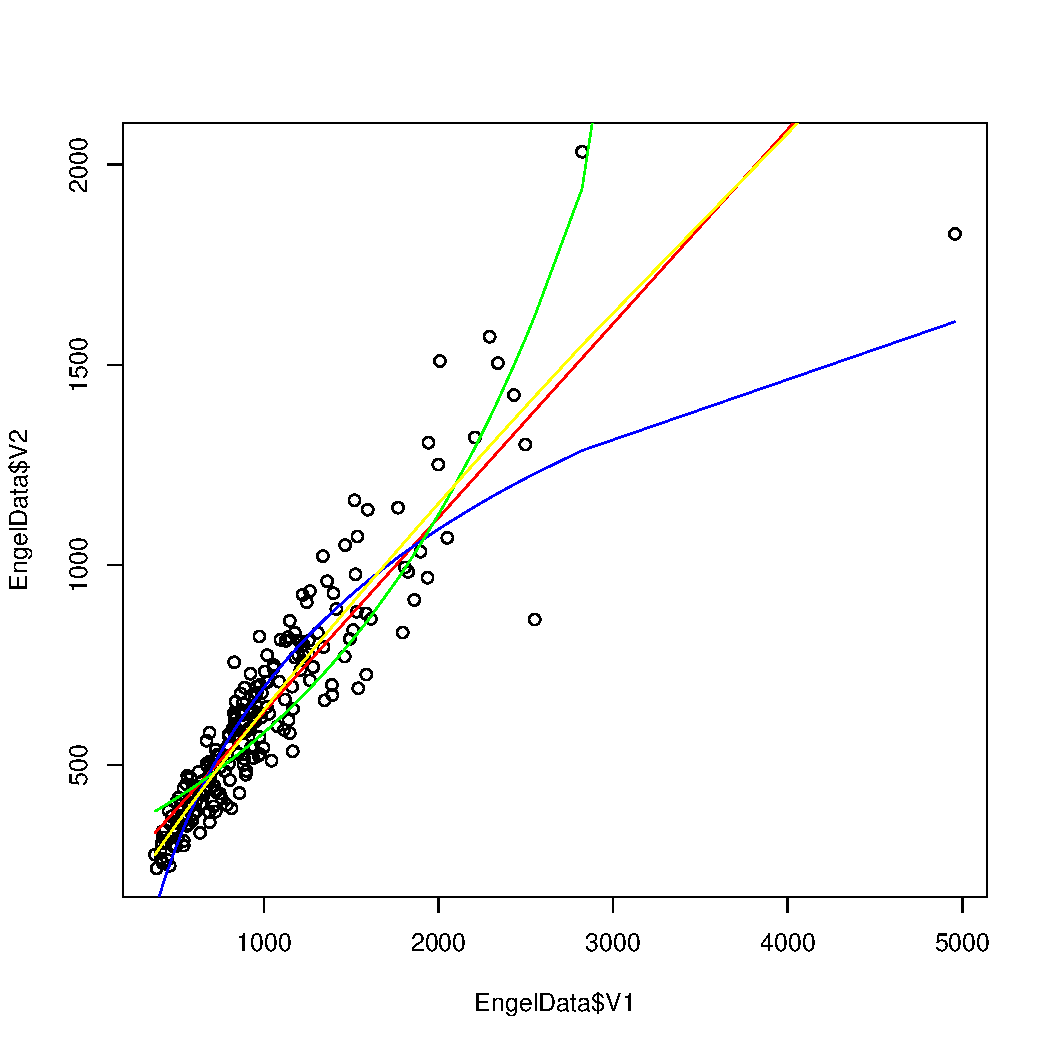
\includegraphics[width=\maxwidth]{figure/q1b-1} 

\end{knitrout}

\section*{c}

We can see that if we take the limit as $\lambda$ tends towards zero,
$\frac{Y_n^\lambda -1 }{\lambda}$ tends to $\log( Y_n )$, so letting $\lambda$ tend
towards zero gives us the log in the Ys and letting $\lambda = 1$ gives us
the standard form. The same can be done for $\psi$ to obtain $\log(x_n)$
enabling us to nest all of these specifications in one model. We can
see this because:
\begin{align*}
  \frac{\alpha^\beta-1}{\beta} = \frac{ \exp{ \beta \log{ \alpha } } -1 }{\beta} = \\
  \frac{( 1 + \beta \log{ \alpha } + \frac{\beta^2}{2} \log{ \alpha }^2 + ... - 1}{\beta} \\
  \log{ \alpha } + \frac{\beta}{2} \log{ \alpha }^2 + ... \\
\end{align*}
Taking the limit as $\beta$ tends towards zero, we see that this
simplifies to $\log{\alpha}$.

To test the different specifications from part b, we would take the
liklihood with nothing imposed upon $\lambda, \psi$ and calculate the liklihood
under the estimated models, twice the difference between those two
would be distributed $\chi^2 (1)$ and from this we could test the
hypothesis that those models are acceptable cases of the Box-Cox
transformation.

This introduces a problem, that we are merely testing if under the
assumption that the Box-Cox Transformation captures the data, then
these function forms are appropiate, not if they are appropiate given
only the data. We have imposed a function form upon the data that
affects our hypothesis testing. One possible way to get around this
problem is to use non-parametrics and a kernal smoothed density
function.

\subsection*{d}


\begin{knitrout}
\definecolor{shadecolor}{rgb}{0.969, 0.969, 0.969}\color{fgcolor}\begin{kframe}
\begin{alltt}
\hlkwd{plot}\hlstd{( EngelData}\hlopt{$}\hlstd{V1, EngelData}\hlopt{$}\hlstd{V2 )}
\hlcom{#Using our previous bandwidth estimates gave us some really bad stuff, so im sticking to .25}
\hlstd{SmoothBoy} \hlkwb{<-} \hlkwd{ksmooth}\hlstd{(} \hlkwd{log}\hlstd{(EngelData}\hlopt{$}\hlstd{V1),} \hlkwd{log}\hlstd{(EngelData}\hlopt{$}\hlstd{V2),}
                     \hlkwc{bandwidth}\hlstd{=}\hlnum{.25}\hlstd{,} \hlkwc{kernel}\hlstd{=}\hlstr{"normal"}\hlstd{,} \hlkwc{x.points} \hlstd{=} \hlkwd{log}\hlstd{(EngelData}\hlopt{$}\hlstd{V1) )}
\hlstd{xweight} \hlkwb{<-} \hlkwd{exp}\hlstd{( SmoothBoy}\hlopt{$}\hlstd{x )}
\hlstd{yweight} \hlkwb{<-} \hlkwd{exp}\hlstd{( SmoothBoy}\hlopt{$}\hlstd{y )}
\hlkwd{lines}\hlstd{(xweight, yweight,} \hlkwc{col}\hlstd{=}\hlstr{"red"}\hlstd{)}
\end{alltt}
\end{kframe}
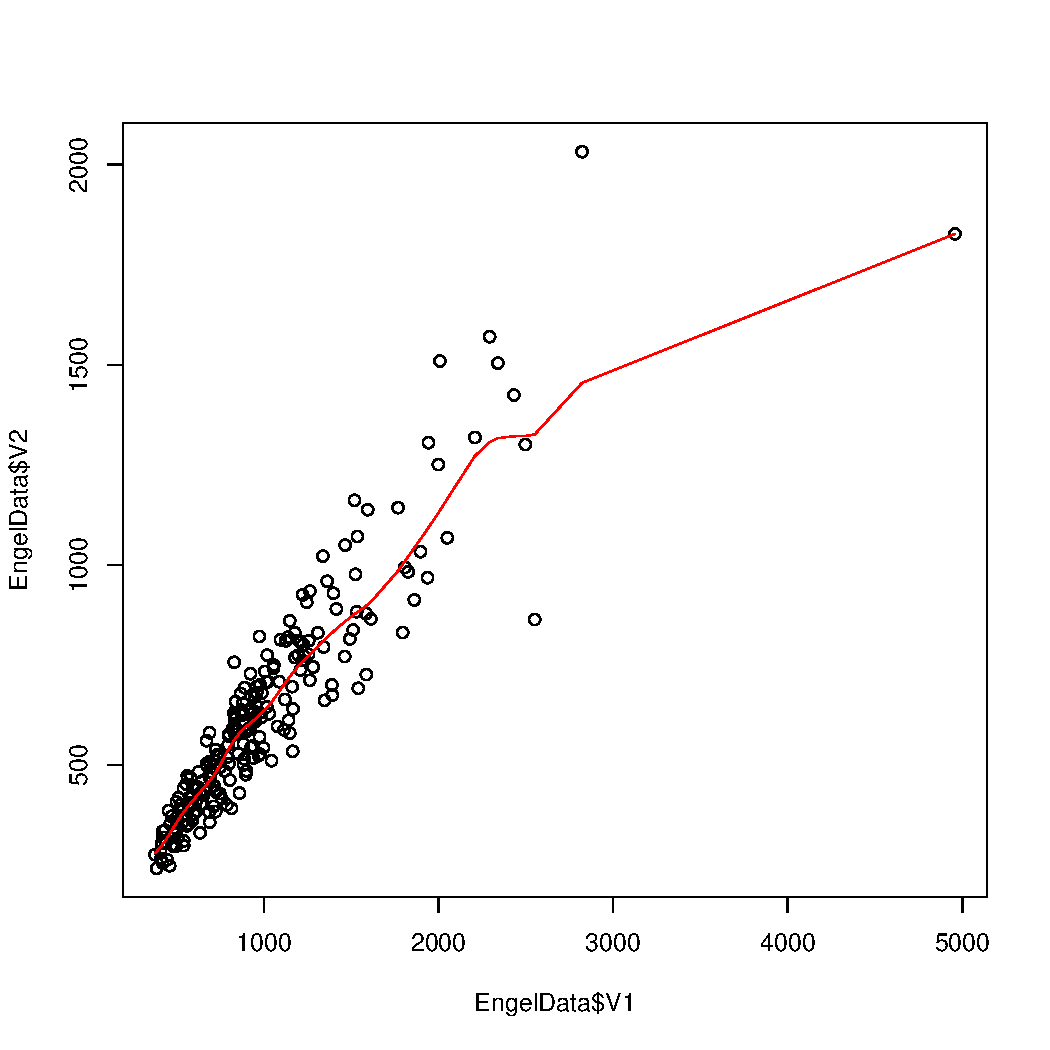
\includegraphics[width=\maxwidth]{figure/unnamed-chunk-2-1} 
\begin{kframe}\begin{alltt}
\hlstd{residuals} \hlkwb{<-} \hlstd{(SmoothBoy}\hlopt{$}\hlstd{y} \hlopt{-} \hlstd{logBoth}\hlopt{$}\hlstd{coefficients[}\hlnum{1}\hlstd{]} \hlopt{-}
              \hlstd{logBoth}\hlopt{$}\hlstd{coefficients[}\hlnum{2}\hlstd{]}\hlopt{*}\hlstd{SmoothBoy}\hlopt{$}\hlstd{x)}

\hlkwd{summary}\hlstd{( residuals )}
\end{alltt}
\begin{verbatim}
##       Min.    1st Qu.     Median       Mean    3rd Qu.       Max. 
## -0.3172000 -0.0050960  0.0027230  0.0002791  0.0128900  0.0344900
\end{verbatim}
\begin{alltt}
\hlkwd{hist}\hlstd{( residuals )}
\end{alltt}
\end{kframe}
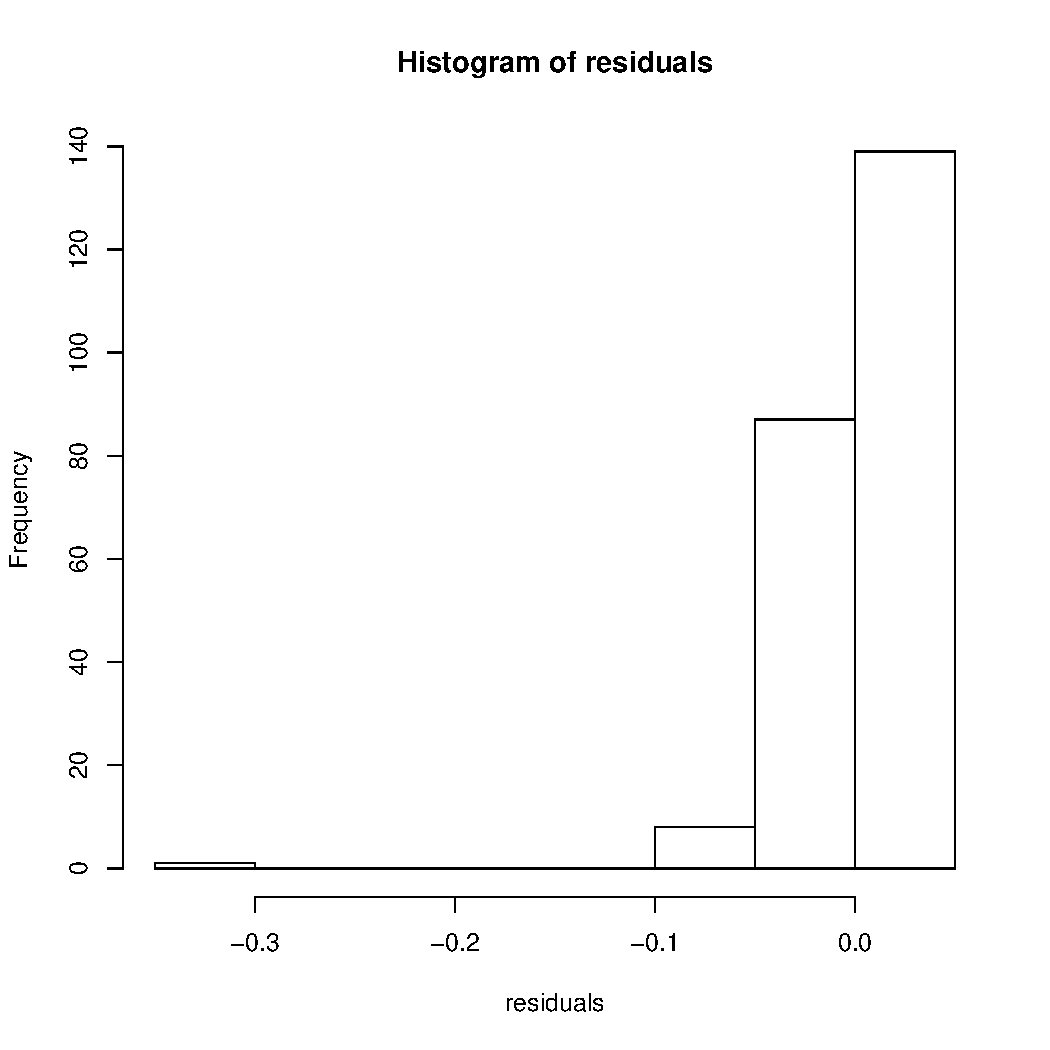
\includegraphics[width=\maxwidth]{figure/unnamed-chunk-2-2} 

\end{knitrout}
If we believe that the Non-parametric estimate is equal to the truth
plus some error term, and under the null hypothesis we believe that
$\log{ y_n } = \hat{\alpha} + \hat{\beta} + U_n$ then our residuals must be
equal to the sum of these two error terms. Given that both error terms
are normal, we can simply apply a test of normality to the residuals. 
 

\begin{knitrout}
\definecolor{shadecolor}{rgb}{0.969, 0.969, 0.969}\color{fgcolor}\begin{kframe}
\begin{alltt}
\hlkwd{shapiro.test}\hlstd{(residuals)}
\end{alltt}
\begin{verbatim}
## 
## 	Shapiro-Wilk normality test
## 
## data:  residuals
## W = 0.62808, p-value < 2.2e-16
\end{verbatim}
\end{kframe}
\end{knitrout}

Based on this p-value we find that the non-parametric regression
rejects the null hypothesis that the model is a valid fit.
\end{document}
